\subsection{Ausgabefenster}
\begin{center}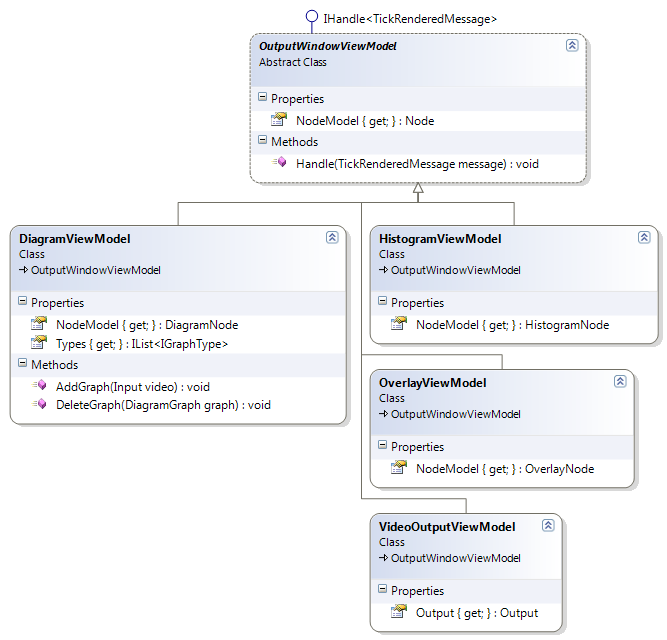
\includegraphics[scale=0.7]{YuvKA.ViewModel/outputs.png} \\
\end{center}
Die abstrakte Klasse \name{OutputWindowViewModel} und ihre konkreten Implementierungen stellen die Daten für die verschiedenen Ausgabefenster, die aus der Hauptoberfläche heraus geöffnet werden können, bereit.

\subsubsection{YuvKA.ViewModel.OutputWindowViewModel}

\begin{verbatim}
public abstract	class OutputWindowViewModel : IHandle<TickRenderedMessage>
\end{verbatim}

\paragraph{Beschreibung}~\\
Die \name{OutputWindowViewModel}-Klasse hält das \name{Node}-Objekt, das die anzuzeigenden Daten enthält, und reagiert auf \name{TickRenderedMessage}s, die vom \name{PipelineState} verschickt werden.

\paragraph{Typmember}
\begin{itemize}

\property{NodeModel}
	\begin{verbatim}
public Node NodeModel { get; }
	\end{verbatim}
	\name{Node}-Objekt, das die anzuzeigenden Daten enthält	

\method{Handle}
	\begin{verbatim}
public virtual void Handle(TickRenderedMessage message)
	\end{verbatim}
	Aktualisiert das Ausgabefenster nach Rendern eines Pipeline-Ticks. Die Standardimplementierung ist leer.

\end{itemize}

\subsubsection{YuvKA.ViewModel.DiagramViewModel}

\begin{verbatim}
public class DiagramViewModel : OutputWindowViewModel
\end{verbatim}

\paragraph{Beschreibung}~\\
Die \name{DiagramViewModel}-Klasse repräsentiert das Ausgabefenster eines \name{DiagramNode}s.

\paragraph{Typmember}
\begin{itemize}

\property{NodeModel}
	\begin{verbatim}
public DiagramNode NodeModel { get; }
	\end{verbatim}
	\name{OutputWindowViewModel.NodeModel}, spezifiziert auf \name{DiagramNode}

\property{Types}
	\begin{verbatim}
public IList<IGraphType> Types { get; }
	\end{verbatim}
	Ermittelt die dynamisch erweiterbare Menge der \name{IGraphType}-Ableitungen und ruft für jede dieser Subklassen eine Instanz ab.

\method{AddGraph}
	\begin{verbatim}
public void AddGraph(Node.Input video)
	\end{verbatim}
	Fügt \name{NodeModel.Graphs} ein neues \name{DiagramGraph}-Objekt mit dem angegebenen Eingabevideo hinzu.

\method{DeleteGraph}
	\begin{verbatim}
public void DeleteGraph(DiagramGraph graph)
	\end{verbatim}
	Löscht den angegebenen Graph aus \name{NodeModel.Graphs}.


\end{itemize}

\subsubsection{YuvKA.ViewModel.HistogramViewModel}

\begin{verbatim}
public class HistogramViewModel : OutputWindowViewModel
\end{verbatim}

\paragraph{Beschreibung}~\\
Die \name{HistogramViewModel}-Klasse repräsentiert das Ausgabefenster eines \name{HistogramNode}s.

\paragraph{Typmember}
\begin{itemize}

\property{NodeModel}
	\begin{verbatim}
public Node NodeModel { get; }
	\end{verbatim}
	\name{OutputWindowViewModel.NodeModel}, spezifiziert auf \name{HistogramNode}

\end{itemize}

\subsubsection{YuvKA.ViewModel.OverlayViewModel}

\begin{verbatim}
public class OverlayViewModel : OutputWindowViewModel
\end{verbatim}

\paragraph{Beschreibung}~\\
Die \name{OverlayViewModel}-Klasse repräsentiert das Ausgabefenster eines \name{OverlayNode}s.

\paragraph{Typmember}
\begin{itemize}

\property{NodeModel}
	\begin{verbatim}
public Node NodeModel { get; }
	\end{verbatim}
	\name{OutputWindowViewModel.NodeModel}, spezifiziert auf \name{OverlayNode}

\end{itemize}

\subsubsection{YuvKA.ViewModel.VideoOutputViewModel}

\begin{verbatim}
public class VideoOutputViewModel : OutputWindowViewModel
\end{verbatim}

\paragraph{Beschreibung}~\\
Die \name{VideoOutputViewModel}-Klasse repräsentiert das Ausgabefenster eines einzelnen Knotenausgangs.

\begin{itemize}

\property{Output}
	\begin{verbatim}
	public Node.Output Output { get; }
	\end{verbatim}
	Ruft den \name{Node.Output} ab, dessen Frameausgabe angezeigt werden soll.

\end{itemize}
